A tweeter can only handle high notes: low notes, with their large amplitudes, would destroy it. A capacitor in series keeps them away. The tweeter acts like a resistor $R$; below the crossover frequency $f_c$, where the reactance of the capacitor equals $R$, the capacitor blocks. The graph shows the measured impedance of tweeter and capacitor together.

\begin{center}
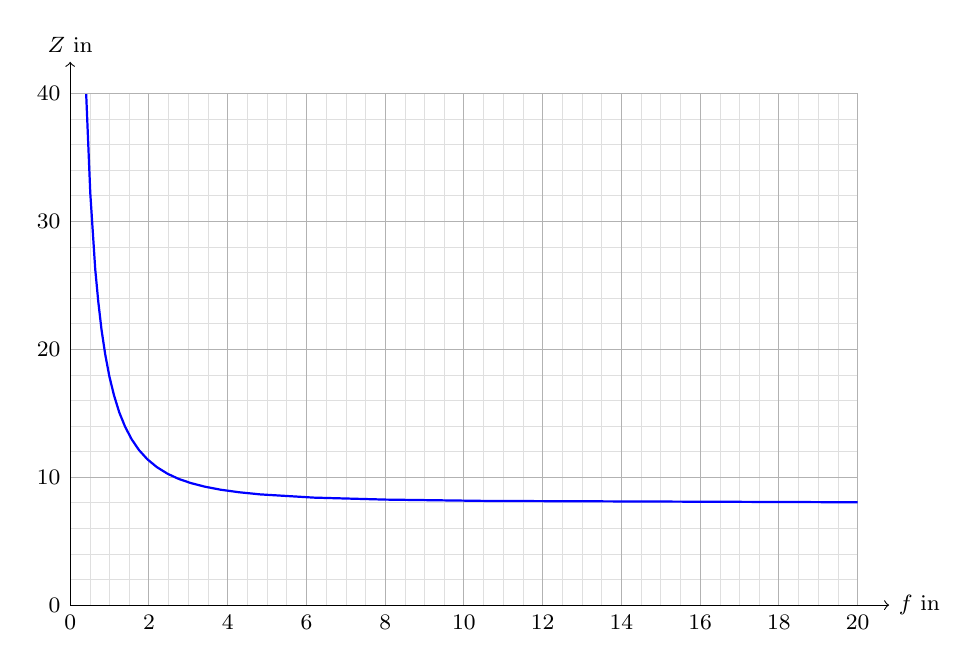
\begin{tikzpicture}[font=\footnotesize]
 \draw[gray!25, very thin] (0.250,0) -- (0.250,6.500) (0.500,0) -- (0.500,6.500) (0.750,0) -- (0.750,6.500) (1.250,0) -- (1.250,6.500) (1.500,0) -- (1.500,6.500) (1.750,0) -- (1.750,6.500) (2.250,0) -- (2.250,6.500) (2.500,0) -- (2.500,6.500) (2.750,0) -- (2.750,6.500) (3.250,0) -- (3.250,6.500) (3.500,0) -- (3.500,6.500) (3.750,0) -- (3.750,6.500) (4.250,0) -- (4.250,6.500) (4.500,0) -- (4.500,6.500) (4.750,0) -- (4.750,6.500) (5.250,0) -- (5.250,6.500) (5.500,0) -- (5.500,6.500) (5.750,0) -- (5.750,6.500) (6.250,0) -- (6.250,6.500) (6.500,0) -- (6.500,6.500) (6.750,0) -- (6.750,6.500) (7.250,0) -- (7.250,6.500) (7.500,0) -- (7.500,6.500) (7.750,0) -- (7.750,6.500) (8.250,0) -- (8.250,6.500) (8.500,0) -- (8.500,6.500) (8.750,0) -- (8.750,6.500) (9.250,0) -- (9.250,6.500) (9.500,0) -- (9.500,6.500) (9.750,0) -- (9.750,6.500);
 \draw[gray!25, very thin] (0,0.325) -- (10.000,0.325) (0,0.650) -- (10.000,0.650) (0,0.975) -- (10.000,0.975) (0,1.300) -- (10.000,1.300) (0,1.950) -- (10.000,1.950) (0,2.275) -- (10.000,2.275) (0,2.600) -- (10.000,2.600) (0,2.925) -- (10.000,2.925) (0,3.575) -- (10.000,3.575) (0,3.900) -- (10.000,3.900) (0,4.225) -- (10.000,4.225) (0,4.550) -- (10.000,4.550) (0,5.200) -- (10.000,5.200) (0,5.525) -- (10.000,5.525) (0,5.850) -- (10.000,5.850) (0,6.175) -- (10.000,6.175);
 \draw[gray!60, thin] (0.000,0) -- (0.000,6.500) (1.000,0) -- (1.000,6.500) (2.000,0) -- (2.000,6.500) (3.000,0) -- (3.000,6.500) (4.000,0) -- (4.000,6.500) (5.000,0) -- (5.000,6.500) (6.000,0) -- (6.000,6.500) (7.000,0) -- (7.000,6.500) (8.000,0) -- (8.000,6.500) (9.000,0) -- (9.000,6.500) (10.000,0) -- (10.000,6.500);
 \draw[gray!60, thin] (0,0.000) -- (10.000,0.000) (0,1.625) -- (10.000,1.625) (0,3.250) -- (10.000,3.250) (0,4.875) -- (10.000,4.875) (0,6.500) -- (10.000,6.500);
 \node[below] at (0.000,0) {0};
 \node[below] at (1.000,0) {2};
 \node[below] at (2.000,0) {4};
 \node[below] at (3.000,0) {6};
 \node[below] at (4.000,0) {8};
 \node[below] at (5.000,0) {10};
 \node[below] at (6.000,0) {12};
 \node[below] at (7.000,0) {14};
 \node[below] at (8.000,0) {16};
 \node[below] at (9.000,0) {18};
 \node[below] at (10.000,0) {20};
 \node[left] at (0,0.000) {0};
 \node[left] at (0,1.625) {10};
 \node[left] at (0,3.250) {20};
 \node[left] at (0,4.875) {30};
 \node[left] at (0,6.500) {40};
 \draw[->] (0,0) -- (10.400,0) node[right] {$f$ in \si{\kilo\hertz}};
 \draw[->] (0,0) -- (0,6.900) node[above] {$Z$ in \si{\ohm}};
 \draw[thick, blue] plot coordinates {(0.203,6.490) (0.255,5.234) (0.318,4.265) (0.357,3.851) (0.398,3.496) (0.445,3.183) (0.498,2.902) (0.557,2.662) (0.623,2.448) (0.697,2.266) (0.780,2.107) (0.873,1.970) (0.980,1.852) (1.100,1.753) (1.237,1.668) (1.375,1.604) (1.532,1.550) (1.710,1.504) (1.914,1.465) (2.147,1.433) (2.415,1.406) (3.096,1.365) (4.002,1.340) (5.288,1.323) (10.000,1.306)};
\end{tikzpicture}
\end{center}

\begin{abcliste}
\abc What is $R$?
\abc What is the crossover frequency?
\abc The woofer plays the notes up to \fxO. Which capacitor puts the crossover there?
\end{abcliste}
